\section{Campo magnetico}
\subsection{Legge di Biot e Savart}
Regola simile a quella del campo elettrico di Coulomb ma applicabile
al campo magnetico.
La formula è:
\begin{equation}
    d\vec{B} = \frac{\mu_0}{4\pi}\frac{Id\vec{l}\times\hat{r}}{r^2}
\end{equation}

Dove si usa la regola della mano destra pe rvedere la direzione 
e si usa la seguante formula per l'intensità:
\begin{equation}
    dB = \frac{\mu_0}{4\pi}\frac{Idl\sin\theta}{r^2}
\end{equation}

\subsection{Permeabilità magnetica del vuoto}
\begin{equation}
    \mu_0 = 4\pi \times 10^{-7} [TmA^{-1}]
\end{equation}

\subsection{Lungo filo percorso da corrente}
Si usa:
\begin{equation}
    B = \frac{\mu_0 I}{2\pi R}
\end{equation}

\subsection{Spira percorsa da corrente}
\begin{figure}[H]
    \centering
    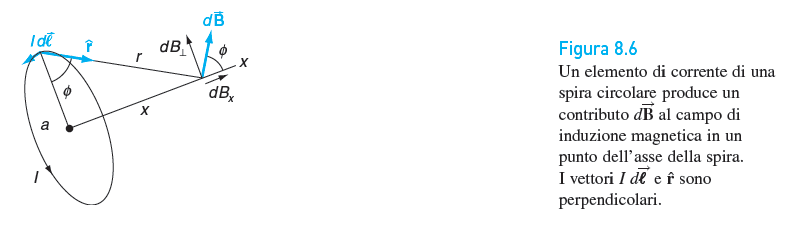
\includegraphics[width=0.5\linewidth]{imgs/13 - spira.png}
    \label{fig:spira_corrente}
    \caption{Spira percorsa da corrente}
\end{figure}
\begin{equation}
    B = \frac{\mu_IS}{2\pi(x^2+a^2)^{\frac{3}{2}}}
\end{equation}

\subsection{Legge di Ampère}
Legge usata per collegare campo magnetico e corrente concatenata.
La formula di base è:
\begin{equation*}
    B = B_1 + B_2 + ... + B_n
\end{equation*}
\begin{equation*}
    B = \sum_i{\frac{\mu_0Il_i}{2\pi R_i}}
\end{equation*}
Però spesso si cambia la lunghezza del'arco e il suo raggio con un angolo:
\begin{equation}
    B = \sum_i{\frac{\mu_0I}{2\pi}\theta_i}
\end{equation}
Questo fa capire che se l'angolo è 0, il risultato è 0(segmenti radiali non contribuiscono)

Se ho un caso dove ho più cerchi concentrici con raggi diversi, 
devo semplicemente sommare i loro contributi,
però prima devo sistemare il fatto che a raggi diverso hanno diverse intnesità.
Quindi se ho due curve, che hanno raggio1 e raggio 2,
\begin{equation*}
    B_2l_2-B_1l_1 = \frac{\mu_0I}{2\pi R_2}R_2\theta - 
    \frac{\mu_0I}{2\pi R_1}R_1\theta
\end{equation*}
Facendo così escludo i raggi dall'equazione.

\subsection{Legge della circuitazione di Ampère}
\begin{figure}[H]
    \centering
    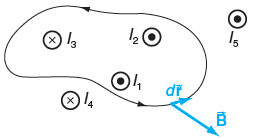
\includegraphics[width=0.3\linewidth]{imgs/14 - cortocircuitazione di ampere.png}
    \label{fig:cortocircuitazione_ampere}
    \caption{Cortocircuitazione di ampere}
\end{figure}

I4 e I5 non sono concatenate con il percorso chiuso, quindi non le considero.
Usanod la regola della mano destra attribuisco i segni alle correnti,
\begin{equation*}
    I_{conc} = I_1 + I_2 - I_3
\end{equation*}

\subsection{Legge di Ampère Vs legge di Gauss}
\begin{itemize}
    \item Ampère: campi magnetici
    \item Coulomb: campi elettrici
\end{itemize}

\subsection{Applicazione di Ampère}
Se cerco il valore esterno al lungo filo rettilineo:
\begin{equation}
    B = \frac{\mu_0I}{2\pi R}
\end{equation}

per R(distanza dal filo al punto) $>$ a(raggio del filo) e 
se il punto è sulla superficie del filo ($R=a$)

Se invece cerco il valore interno al filo:
\begin{equation}
    B = \frac{\mu_0}{2\pi R}I\frac{R^2}{a^2} = \frac{\mu_0IR}{2\pi a^2}
\end{equation}

\subsection{Campo magnetico di un solenoide}
Il solenoide ha lacaratteristica di produrre un campo tendente al nullo
all'esterno e un campo uniforme all'interno delle spire.
Maggiore è la lunghezza è il numero di spire, migliore è il risultato della 
concatenzaione.

Per trovare Il campo magnetico all'interno del solenoide, si usa La
legge di Ampère del percorso chiuso e l'unico campo non zero è quello all'interno.
Per cui vale la formula:
\begin{equation}
    B = \mu_0nI
\end{equation}
Dove $n=\frac{N}{L}$ dove rispettivamente L è la lunghezza ed N è il numero di spire.
Così facendo, si ottiene $n$ che è il numero di spire in unità di spazio.


\subsection{Forza agente tra conduttori}
Se ho due fili attraversati da corrente con segno opposto, si attraggono 
con la seguente forza:
\begin{equation}
    F = \frac{\mu_0I_1I_2}{2\pi R}l
\end{equation}
Se hanno stesso verso, si respingono con la stessa forza.
R è la distanza tra i due fili ed l è la lunghezza considerata.

\subsection{Flusso magnetico}
Come per il campo elettrico, esiste un flusso elettrico, per il campo 
magnetico esiste il flusso magnetico.
\begin{equation}
    \phi_B = \iint_S{B\cos\theta \cdot dS}
\end{equation}

L'unità di misura è il Weber(Wb), $1Wb = 1Tm^{2}$.


\subsection{Legge di Gauss per il campo elettrico}
\begin{equation*}
    \phi_E = \frac{Q_{int}}{\epsilon_0}
\end{equation*}

\subsection{Legge di Gauss per il campo magnetico}
\begin{equation*}
    \phi_B = \oiint{\vec{B}\cdot d\vec{S}}
\end{equation*}

Il flusso magnetico attraverso una superficie chiusa è nullo.


\subsection{Modifica della legge di Ampère}

\begin{figure}[H]
    \centering
    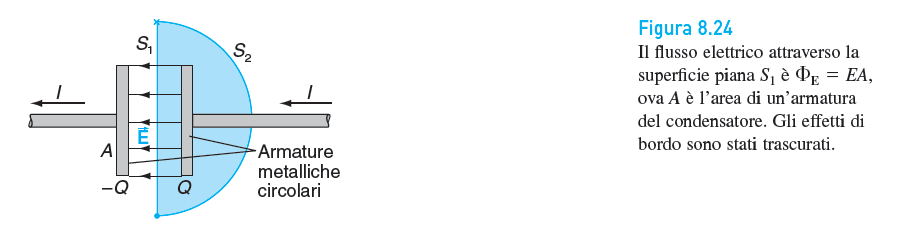
\includegraphics[width=0.8\linewidth]{imgs/16 - ampere modificata da maxwell.png}
    \label{fig:ampere_modificata}
    \caption{Ampèere modificata da Maxwell}
\end{figure}

La legge di Ampère:
\begin{equation*}
    \oint{\vec{B}\cdot d\vec{r}} = \mu_0I_{conc}
\end{equation*}
La modifica di Maxwell è:
\begin{equation}
    E = \frac{|\sigma|}{\epsilon_0} = \frac{Q}{\epsilon_0A}
\end{equation}
dove epsilon è la densità di carica dell'armatura.


\begin{equation}
    \phi_E = EA
\end{equation}
risolvendo rispetto a Q:
\begin{equation}
    Q = \epsilon_0 EA = \epsilon_0\phi_E
\end{equation}
Poi, derivando il tutto si ottiene:
\begin{equation}
    I = \frac{dQ}{dt} = \epsilon_0\frac{d\phi_E}{dt}
\end{equation}


La corrente I atraversa S2, la corrente di spostamento
IS attraversa S1 ed I=IS.

\subsection{Legge di Ampère modificata}
\begin{equation}
    \oint{\vec{B}\cdot d\vec{r}} = \mu_0\Bigg(I_{conc} + 
    \epsilon_0\frac{d\phi_E}{dt}\Bigg)
\end{equation}